\documentclass{article}

\usepackage[T1]{fontenc}
\usepackage[utf8]{inputenc}
\usepackage{graphicx}
\usepackage{polski}
\usepackage{listings}
\usepackage{xcolor}

\colorlet{punct}{red!60!black}
\definecolor{background}{HTML}{EEEEEE}
\definecolor{delim}{RGB}{20,105,176}
\colorlet{numb}{magenta!60!black}

\newcommand{\mparagraph}[1]{\paragraph{#1}\mbox{}\vspace{2mm}\\}

\lstdefinelanguage{json}{
    basicstyle=\normalfont\ttfamily,
    numbers=left,
    numberstyle=\scriptsize,
    stepnumber=1,
    numbersep=8pt,
    showstringspaces=false,
    breaklines=true,
    frame=lines,
    literate=
     *{0}{{{\color{numb}0}}}{1}
      {1}{{{\color{numb}1}}}{1}
      {2}{{{\color{numb}2}}}{1}
      {3}{{{\color{numb}3}}}{1}
      {4}{{{\color{numb}4}}}{1}
      {5}{{{\color{numb}5}}}{1}
      {6}{{{\color{numb}6}}}{1}
      {7}{{{\color{numb}7}}}{1}
      {8}{{{\color{numb}8}}}{1}
      {9}{{{\color{numb}9}}}{1}
      {:}{{{\color{punct}{:}}}}{1}
      {,}{{{\color{punct}{,}}}}{1}
      {int}{{{\color{magenta}{int}}}}{3}
      {string}{{{\color{magenta}{string}}}}{6}
      {boolean}{{{\color{magenta}{boolean}}}}{7}
      {"}{{{\color{numb}{"}}}}{1}
      {\{}{{{\color{delim}{\{}}}}{1}
      {\}}{{{\color{delim}{\}}}}}{1}
      {[}{{{\color{delim}{[}}}}{1}
      {]}{{{\color{delim}{]}}}}{1},
}

\title{Specyfikacja implementacyjna - Poker Royal Flush}
\author{Artur Prasuła}

\begin{document}
\maketitle
\tableofcontents
\newpage


\section{Opis API} % 25.03
    API wykorzystywane jest do komunikacji pomiędzy aplikacją serwerową, a aplikacją kliencką.
    Komunikaty wykorzystują format JSON. Każdy z typów komunikatów ma swoją nazwę, która informuje o zastosowaniu danego komunikatu.
    
    \subsection{Komunikat start}
        Komunikat \textbf{start} wysyłany jest przez serwer do klienta.
        Informuje on o rozpoczęciu nowej rundy oraz przesyła informacje o wylosowanych dwóch kartach dla każdego gracza.
        \begin{lstlisting}[language=json,firstnumber=1]
{
    "name": "start",
    "cards": [
        {"number": int, "color": int},
        {"number": int, "color": int}
    ]
}
        \end{lstlisting}
    
    \subsection{Komunikat info}
        Komunikat \textbf{info} wysyłany jest przez serwer do wszystkich klientów, po każdej zmianie stanu stołu.
        Dzięki temu w aplikacji klienckiej stół zawsze jest aktualny.
    
        \begin{lstlisting}[language=json,firstnumber=1]
{
    "name": "info",
    "table": {
        "cards":[
            {"number": int, "color": int},
            {"number": int, "color": int},
            {"number": int, "color": int}
        ],
        "pot": int,
        "players": [
            {
                "nickname": string,
                "money": int,
                "state": int,
                "pot": int
            },
            {
                "nickname": string,
                "money": int,
                "state": int,
                "pot": int
            }
        ]
    }
}
        \end{lstlisting}
        Liczba kart w sekcji \textbf{cards} zawiera się w przedziale <0;5>.\\
        Liczba graczy w sekcji \textbf{players} zawiera się w przedziale <1;6>.
    
    \subsection{Komunikat request}
        Komunikat \textbf{request} wysyłany jest przez serwer do klienta.
        Jest to żądanie wykonania ruchu przez gracza do którego to żądanie jest wysyłane.
        Serwer po wysłaniu tego komunikatu, nasłuchuje wiadomości zwrotnej od klienta.
    
        \begin{lstlisting}[language=json,firstnumber=1]
{
    "name": "request",
    "minValue": int
}
        \end{lstlisting}
        Wartość \textbf{minValue} oznacz minimalną ilość pieniędzy jaką gracz musi dołożyć do puli.
    
    \subsection{Komunikat end}
        Komunikat \textbf{end} wysyłany jest przez serwer do klienta.
        Informuje on o zakończeniu rundy oraz o informacjach związanych z końcem: zwycięzca/y, wysokość wygranej, karty graczy.
        \begin{lstlisting}[language=json,firstnumber=1]
{
    "name": "end",
    "prize": int,
    "players": [
        {
            "nickname": string,
            "winner": boolean,
            "cards": [
                {"number": int, "color": int},
                {"number": int, "color": int}
            ]
        },
        {
            "nickname": string,
            "winner": boolean,
            "cards": [
                {"number": int, "color": int},
                {"number": int, "color": int}
            ]
        }
    ]
}
        \end{lstlisting}
        Liczba graczy w sekcji \textbf{players} zawiera się w przedziale <1;4>.
    
    \subsection{Komunikat move}
        Komunikat \textbf{move} jest jedynym komunikatem wysyłanym przez klienta do serwera.
        Informuje on o wykonanym przez gracza ruchu.
        Z powodu tego, że możliwe ruchy są od siebie różne, komunikaty \textbf{move} można pogrupować ze względu na typ ruchu: call, fold, check, raise.
        
        \subsubsection{Call, Fold, Check}
            \begin{lstlisting}[language=json,firstnumber=1]
{
    "name": "move",
    "type": int
}
            \end{lstlisting}
            Wartość \textbf{type} mówi o typie komunikatu. Wysyłane wartości tego atrybutu powinny być zgodne z tym co przechowuje klasa \textbf{poker.properties.PlayerMoveProperties}.

        \subsubsection{Raise}
            \begin{lstlisting}[language=json,firstnumber=1]
{
    "name": "move",
    "type": 3,
    "value": int
}
            \end{lstlisting}


\section{Opis pakietu properties}
    Pakiet \textbf{poker.properties} odpowiada za przechowywanie stałych wspólnych dla części klienckiej i części serwerowej.
    Znajdziemy w nim klasy: CardsProperties, PlayerMoveProperties, PlayerStateProperties.
    
    \subsection{Klasa CardsProperties}
        Klasa \textbf{CardsProperties} przechowuje liczby całkowite, które odpowiadają kolorom kart.
        \paragraph{Pola}
            \begin{itemize}
                \item public static final int CLUBS = 0
                \item public static final int DIAMONDS = 13
                \item public static final int HEARTS = 26
                \item public static final int SPADES = 39
            \end{itemize}
            
    \subsection{Klasa PlayerMoveProperties}
        Klasa \textbf{PlayerMoveProperties} przechowuje liczby całkowite, które odpowiadają danym ruchom gracza.
        Liczby te zostaną wykorzystane w API w komunikacie \textbf{move}.
        \paragraph{Pola}
            \begin{itemize}
                \item public static final int CALL = 0
                \item public static final int FOLD = 1
                \item public static final int CHECK = 2
                \item public static final int RAISE = 3
            \end{itemize}
    
    \subsection{Klasa PlayerStateProperties}
        Klasa \textbf{PlayerStateProperties} przechowuje liczby całkowite, które odpowiadają danym stanom gracza.
        Liczby te zostaną wykorzystane aby przechowywać informacje o stanie rozgrywki oraz w API w komunikacie \textbf{info}.
        \paragraph{Pola}
            \begin{itemize}
                \item public static final int INGAME = 0
                \item public static final int AFTERFOLD = 1
                \item public static final int INMOVE = 2
            \end{itemize}

\section{Opis części serwerowej}
    \subsection{Opis ogólny}
        Część serwerowa odpowiada za poprawne przeprowadzenie rozgrywki.
        Uruchamiana jest z linii poleceń i nie posiada GUI, gdyż w trakcie działania, nie wymaga ingerencji użytkownika.
    
    \subsection{Diagram klas}
        \begin{center}
            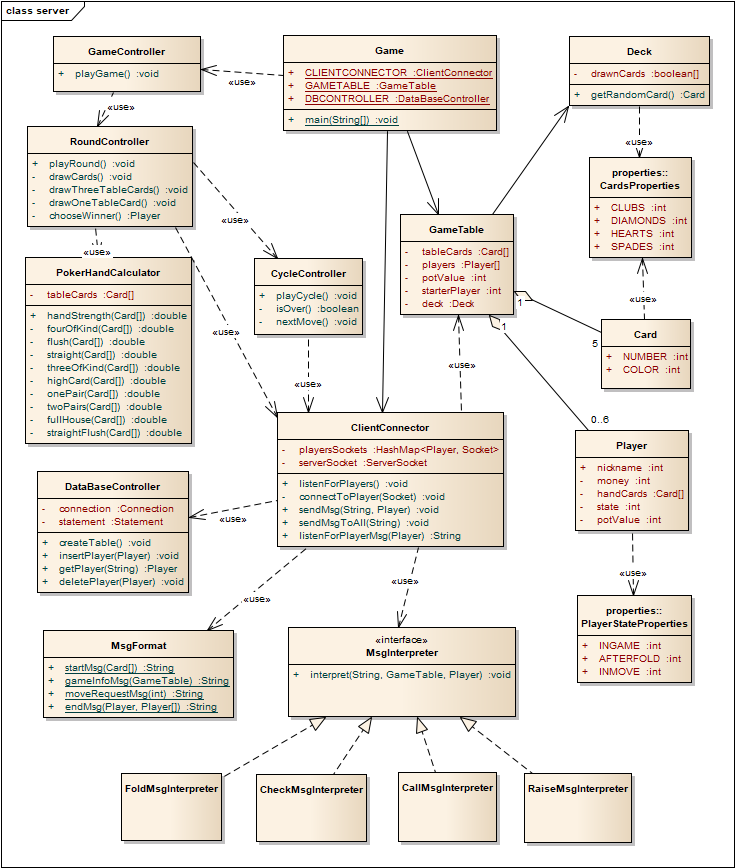
\includegraphics[width=\textwidth]{class_server.png}
        \end{center}
    
    \subsection{Opis pakietów}
        \subsubsection{poker.server}
            Pakiet \textbf{poker.server} odpowiada za część serwerową programu.
        
            \mparagraph{Klasa - Game}
                Klasa \textbf{Game} przechowuje referencje do obiektów, które powstają po uruchomieniu programu i nie zmieniają się aż do końca działania programu.
                Te obiekty wykorzystywane są przez różne klasy, dzięki temu zapewniony jest łatwy dostęp do nich.
                \\
                Metoda \textbf{main} uruchamia komunikację z klientami, tworzy nowy stół do gry, tworzy dostęp do bazy danych i uruchamia rozgrywkę po dołączeniu odpowiedniej liczby graczy.
            
                
        \subsubsection{poker.server.data}
            Pakiet \textbf{poker.server.data} służy do przechowywania danych, związanych z rozgrywką, w pamięci.
        
            \mparagraph{Klasa - GameTable}
                Klasa \textbf{GameTable} służy do przechowywania informacji o aktualnej rozgrywce.
                \\
                W tej klasie znajdziemy tylko metody dostępowe do prywatnych pól.
                
            \mparagraph{Klasa - Player}
                Klasa \textbf{Player} przechowuje informacje o danym graczu.
                Wykorzystuje ona stałe z klasy \textbf{poker.properties.PlayerStateProperties}.
                \\
                W tej klasie są tylko metody dostępowe do prywatnych pól.
        
        \subsubsection{poker.server.data.cards}
        
            \mparagraph{Klasa - Card}
                Klasa \textbf{Card} przechowuje informacje o danej karcie.
                Wykorzystuje ona stałe z klasy \textbf{poker.properties.CardsProperties}.
        
            \mparagraph{Klasa - Deck}
                Klasa \textbf{Deck} przechowuje wszystkie możliwe karty.
                \\
                Pole \textbf{drawnCards} przechowuje informacje o tym, czy dana karta została już wyjęta z talii.
                Karty z danego koloru znajdują się w danym przedziale. Przedział ten odpowiada stałym z klasy \textbf{poker.properties.CardsProperties}. Im (indeks \% kolor) większe, tym wyższa jest to karta.
                \\
                Metoda \textbf{getRandomCard} zwraca losową kartę z talii, ale wykonuje losowanie bez powtórzeń, więc nie da się wyciągnąć z talii dwóch takich samych kart.
            
        
        \subsubsection{poker.server.data.database}
        
            \mparagraph{Klasa - DataBaseController}
                Klasa \textbf{DataBaseController} służy do komunikacji z bazą danych.
                Wykorzystywany system zarządzania bazą danych to PostgreSQL.
                \\
                W klasie znajdują się pola służące do komunikacji z bazą danych.
                \\
                Znajdziemy w niej metody dostępowe do bazy danych takie jak: tworzenie bazy; dodawanie, usuwanie i sprawdzanie gracza.
                
                
        \subsubsection{poker.server.communication}
            Pakiet \textbf{poker.server.communication} służy do komunikacji serwera z klientami.
            
            \mparagraph{Klasa - ClientConnector}
                Klasa \textbf{ClientConnector} służy do połączenia serwera z klientami.
                \\
                Przechowuje ona gniazda sieciowe, które służą do bezpośredniej komunikacji z klientami.
                \\
                Metoda \textbf{listenForPlayers} stale nasłuchuje na dołączenie się nowych graczy.
                W momencie dołączenia, wykonuje się metoda \textbf{connectToPlayer}, która tworzy powiązanie serwera z klientem.
                
            \mparagraph{Klasa - MsgFormat}
                Klasa \textbf{MsgFormat} służy do automatycznego formatowania komunikatów wysyłanych przez serwer.
    
        \subsubsection{poker.server.communication.interpreters}
            Pakiet \textbf{poker.server.communication.interpreters} służy do interpretowania komunikatów \textbf{move} wysyłanych przez klientów.
        
            \mparagraph{Interfejs - MsgInterpreter}
                Interfejs posiada jedną metodę: \textbf{interpret}, która służy do interpretacji komunikatu \textbf{move} i wykonania odpowiednich kroków w zależności od typu komunikatu.
        
            \mparagraph{Klasa - CallMsgInterpreter}
                Klasa \textbf{CallMsgInterpreter} służy do wykonania komunikatu o wykonaniu przez gracza ruchu call - sprawdzenia.
                
            \mparagraph{Klasa - CheckMsgInterpreter}
                Klasa \textbf{CheckMsgInterpreter} służy do wykonania komunikatu o wykonaniu przez gracza ruchu check - czekania.
                
            \mparagraph{Klasa - FoldMsgInterpreter}
                Klasa \textbf{FoldMsgInterpreter} służy do wykonania komunikatu o wykonaniu przez gracza ruchu fold - pasowania.
                
            \mparagraph{Klasa - RaiseMsgInterpreter}
                Klasa \textbf{RaiseMsgInterpreter} służy do wykonania komunikatu o wykonaniu przez gracza ruchu raise - podbicia.
    
        \subsubsection{poker.server.gamecontrollers}
            Pakiet \textbf{poker.server.gamecontrollers} ma za zadanie przeprowadzanie rozgrywki w sposób poprawny i uporządkowany.
            
            \mparagraph{Klasa - GameController}
                Klasa \textbf{GameController} odpowiada za przeprowadzenie ogólnej rozgrywki.
                Sprawdza czy jest poprawna liczba graczy w grze, sprawdza czy gra nie powinna się już skończyć, wywołuje kolejne rundy za pomocą klasy \textbf{RoundController}.
                
            \mparagraph{Klasa - RoundController}
                Klasa \textbf{RoundController} odpowiada za przeprowadzenie pojedynczej rundy od początku do końca, czyli: przetasowanie kart, wylosowanie kart dla każdego z graczy, wylosowanie kart wspólnych, wywoływanie cyklów za pomocą klasy \textbf{CycleController}, wybranie zwycięzcy/ów rundy za pomocą klasy \textbf{PokerHandCalculator}, podział puli.
                
            \mparagraph{Klasa - CycleController}
                Klasa \textbf{CycleController} odpowiada za przeprowadzenie pojedynczego cyklu w trakcie rundy.
                Jej zadania to: żądanie wykonania ruchu przez każdego z graczy, dołączenie nowych pieniędzy do puli.
                
        \subsubsection{poker.server.gamecontrollers.hands}
        
            \mparagraph{Klasa - PokerHandCalculator}
                Klasa \textbf{PokerHandCalculator} oblicza jaki jest najsilniejszy układ z podanych kart.
                Metoda \textbf{handStrength} zwraca liczbę double z zakresu 0-9.
                Każda cyfra jedności odpowiada danemu układowi:
                \begin{itemize}
                    \item 0 - wysoka karta
                    \item 1 - para
                    \item 2 - dwie pary
                    \item 3 - trójka
                    \item 4 - strit
                    \item 5 - kolor
                    \item 6 - full
                    \item 7 - kareta
                    \item 8 - poker
                \end{itemize}
                Może zdarzyć się sytuacja, że dwa układy kart pomimo, że będą to te same układy, będą składać się z różnych kart i będą mieć różną moc. W takiej sytuacji liczba jedności będzie taka sama, ale liczba po przecinku będzie się różnić.
                \\\\
                Ogólna zasada zwracanej liczby jest taka, że jeśli układ A jest silniejszy od układu B, to metoda \textbf{handStrength} zwróci liczby takie, że spełniają zależność: A > B.
                W przypadku gdy układy będą takie same, zwrócone liczby spełnią zależność A = B.

\section{Opis części klienckiej}
    \subsection{Opis ogólny}
        Część kliencka, będzie to część aplikacji, która jest przeznaczona dla zwykłych klientów.
        To za jej pomocą będzie można grać w pokera.
        \\
        Tworzony kod oraz struktura pakietów jest zgodna z wzorcem projektowym MVC.
    
    \subsection{Diagram klas}
        \begin{center}
            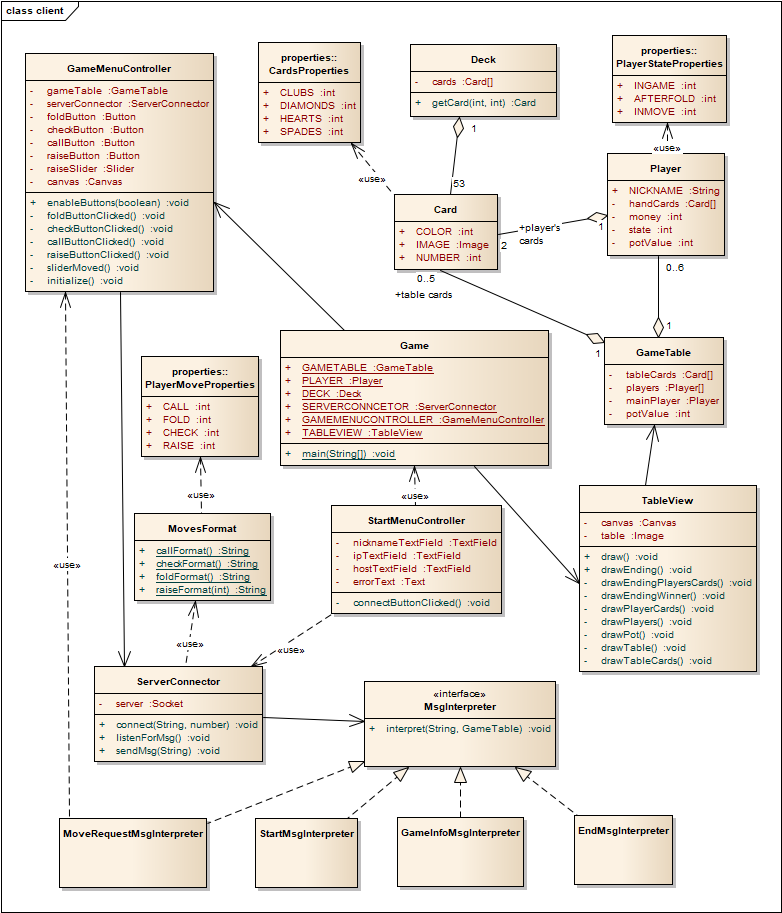
\includegraphics[width=\textwidth]{class_client.png}
        \end{center}
    
    \subsection{Opis pakietów}
        
        \subsubsection{poker.client}
            Pakiet \textbf{poker.client} jest pakietem, który odpowiada za część kliencką aplikacji.
            
            \mparagraph{Klasa - Game}
                Klasa \textbf{Game} przechowuje referencje do obiektów, które wykorzystywane są we wszystkich częściach aplikacji.
                Takie rozwiązanie zapewnia łatwy dostęp do tych obiektów.
                \\
                Metoda \textbf{main} uruchamia część graficzną programu oraz tworzy obiekty, które ta klasa przechowuje.
        
        \subsubsection{poker.client.data}
            Pakiet \textbf{poker.client.data} odpowiada za przechowywanie danych o stole, graczach i kartach w programie.
            
            \mparagraph{Klasa - GameTable}
                Klasa \textbf{GameTable} przechowuje informacje o aktualnej rozgrywce - wspólnych kartach, graczach przy stole, puli w grze. Dodatkowo przechowuje informacje o tym, którym graczem jest użytkownik aplikacji.
            
            \mparagraph{Klasa - Player}
                Klasa \textbf{Player} przechowuje informacje o graczu - pseudonimie, jego kartach, pieniądzach i stanie gracza.
                Do określenia stanu gracza wykorzystywana jest klasa \textbf{poker.properties.PlayerStateProperties}.
            
        \subsubsection{poker.client.data.cards}
        
            \mparagraph{Klasa - Card}
                Klasa \textbf{Card} przechowuje informacje o danej karcie - numer, kolor i zdjęcie karty.
                Do określenia koloru karty wykorzystuje się stałe zawarte w klasie \textbf{poker.properties.CardsProperties}.
            
            \mparagraph{Klasa - Deck}
                Klasa \textbf{Deck} przechowuje talię gotowych kart (nie wymagają one inicjalizacji np. obrazku).
                \\
                Metoda \textbf{getCard} zwraca referencję do gotowego obiektu karty.
            
        \subsubsection{poker.client.communication}
            Pakiet \textbf{poker.client.communication} odpowiada za komunikację części klienckiej z częścią serwerową.
            
            \mparagraph{Klasa - ServerConnector}
                Klasa \textbf{ServerConnector} odpowiada za połączenie między klientem a serwerem.
                Za jej pomocą będzie można komunikat wysłać do serwera albo odebrać go od serwera.
                \\
                Metoda \textbf{listenForMsg} będzie nieustannie wysłuchiwać komunikatów od serwera, a w przypadku odebrania jakiegoś, wykorzysta odpowiednią klasę (w zależności od komunikatu) implementującą interfejs \textbf{interpreteres.MsgInterpreter}.
            
            \mparagraph{Klasa - MovesFormat}
                Klasa \textbf{MovesFormat} odpowiada za zautomatyzowanie tworzenia komunikatów wysyłanych do serwera.
                Klasa do poprawnego zintegrowania komunikatów z serwerem, będzie korzystać ze stałych zawartych w klasie \textbf{poker.properties.PlayerMoveProperties}.
                
        \subsubsection{poker.client.communication.interpreters}
            Pakiet \textbf{poker.client.communication.interpreters} ma za zadanie interpretację odpowiednich komunikatów przysyłanych przez serwer i wykonanie odpowiednich kroków w zależności od komunikatu.
            
            \mparagraph{Interfejs - MsgInterpreter}
                Interfejs posiada jedną metodę: \textbf{interpret}. Metoda ta służy do interpretacji komunikatu i wykonania odpowiednich kroków w zależności od komunikatu.
            
            \mparagraph{Klasa - StartMsgInterpreter}
                Klasa \textbf{StartMsgInterpreter} interpretuje komunikat \textbf{start} - ,,czyści'' stół, daje graczowi odpowiednie karty.
            
            \mparagraph{Klasa - GameInfoMsgInterpreter}
                Klasa \textbf{GameInfoMsgInterpreter} interpretuje komunikat \textbf{info} - aktualizuje dane stołu i graczy zawarte w komunikacie.
            
            \mparagraph{Klasa - MoveRequestMsgInterpreter}
                Klasa \textbf{MoveMoveRequestInterpreter} interpretuje komunikat \textbf{request} - w zależności od zawartych danych w komunikacie, odblokowuje wybrane przyciski, aby użytkownik mógł wykonać ruch.
            
            \mparagraph{Klasa - EndMsgInterpreter}
                Klasa \textbf{EndMsgInterpreter} interpretuje komunikat \textbf{end} - aktualizuje dane stołu i zwycięzców.
            
        \subsubsection{poker.client.controller}
            Pakiet \textbf{poker.client.controller} odpowiada za kontrolę przycisków w GUI - odpowiednie odblokowywanie i zablokowywanie, reagowanie na wciśniecia przycisków i przesunięcia suwaków.
            
            \mparagraph{Klasa - StartMenuController}
                Klasa \textbf{StartMenuController} odpowiada za obsługę kontrolek w oknie startowym aplikacji.
                \\
                Metoda \textbf{connectButtonClicked} inicjuje próbę połączenia się do serwera.
                Gdy próba się uda, okno startowe jest zamykane, a pojawia się okno główne.
                W przeciwnym wypadku, wypisywany jest odpowiedni komunikat do \textbf{errorText}.
            
            \mparagraph{Klasa - GameMenuController}
                Klasa \textbf{GameMenuController} odpowiada za obsługę kontrolek w menu gry w oknie głównym.
                \\
                Metody związane z przyciskami wysyłają odpowiednie komunikaty do serwera za pomocą klas zawartych w pakiecie \textbf{poker.client.communication}.
                \\
                Metoda \textbf{enableButtons} włącza wszystkie przyciski w przypadku podania argumentu wynoszącego \textbf{true}.
                W przeciwnym wypadku metoda nie włącza przycisku \textbf{callButton}.

        \subsubsection{poker.client.view}
            Pakiet \textbf{poker.client.view} odpowiada za widok stołu.
            
            \mparagraph{Klasa - TableView}
                Klasa \textbf{TableView} odpowiada za rysowanie widoku stołu - graczy, puli, kart, wygranej.
                Wykonuje to korzystając z gotowych obrazów stołu i kart.
                
        \subsubsection{resources}
            Katalog \textbf{resources} będzie podzielony na mniejsze katalogi.\\
            Struktura katalogów:
            \begin{verbatim}
    resources
      |- fxml
      |- graphics
           |- cards
              |- 0
              |- 13
              |- 26
              |- 39
            \end{verbatim}
            Katalog \textbf{/resources/fxml/} przechowuje pliki fxml okna startowego i okna głównego.\\
            W katalogu \textbf{/resources/graphics/} znajdują się grafiki stołu, graczy i katalog \textbf{/cards/} w którym zawarte są grafiki kart.\\
            Katalogi kart są podzielone ze względu na kolory.
            Nazwy katalogów w zależności od koloru odpowiadają stałym zawartym w klasie \textbf{poker.properties.CardsProperties}.
            
    \subsection{Opis GUI}
        Graficzny interfejs będzie składać się z 2 okienek.
        Pierwsze okienko będzie uruchamiać się po włączeniu aplikacji i będzie służyć do połączenia się z serwerem.
        Drugie okienko uruchomi się po dołączeniu do serwera.
        Będzie ono odpowiadać za widok stołu, graczy i menu wyboru możliwych ruchów.
        
        \subsubsection{Okno startowe}
        
            \begin{center}
                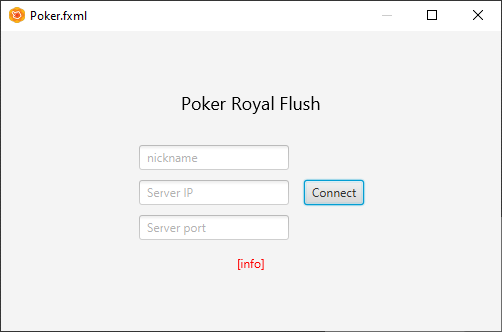
\includegraphics[width=70mm]{gui_start.png}
            \end{center}
        
            Okienko startowe pojawi się na środku ekranu i będzie mieć rozmiary: szerokość - 500,  wysokość - 300.
            Do przycisku \textbf{Connect} będzie podpięty słuchacz akcji, który będzie reagować na wciśnięcie go.
            Po jego wciśnięciu, program na podstawie informacji zawartych w polach: \textbf{nickname, Server IP, Server port} wykona próbę dołączenia się do danego serwera.
            Błędy będą wyświetlane na czerwono w miejscu \textbf{info}.
            \\
            \textbf{Budowa wewnętrzna GUI:}
            \begin{verbatim}
    VBox
      |- Text
      |- HBox
           |- VBox
                |- TextField
                |- TextField
                |- TextField
           |- Button
      |- Text
            \end{verbatim}
        
        \subsubsection{Okno główne}
        
            \begin{center}
                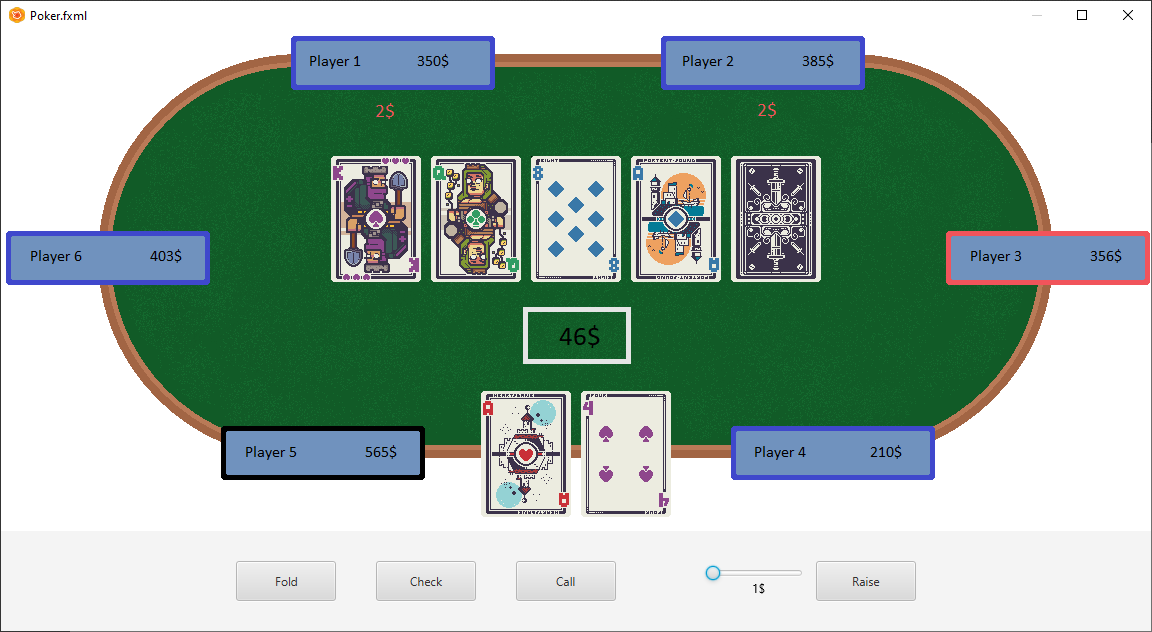
\includegraphics[width=\textwidth]{gui_table.png}
            \end{center}
        
            Okno główne pojawia się w momencie dołączenia do serwera.
            Będzie mieć rozmiar: szerokość - 1150, wysokość - 650.\\
            Panel głównego okna, można podzielić na dwa mniejsze: canvas i menu wyboru ruchów.\\
            Canvas będzie mieć za zadanie wyświetlanie widoku stołu wraz z graczami. Jego szerokość będzie równa 1150, a wysokość będzie równa 500.\\
            Menu wyboru ruchu składa się z kontrolek, które odpowiadają za wykonanie ruchów przez gracza.
            Do każdego z przycisków i suwaka będzie przypisany słuchacz akcji.
            Po wciśnięciu odpowiedniego przycisku, program wyśle do serwera komunikat o tym, jaki ruch został wykonany.
            Słuchacz akcji slider'a będzie nasłuchiwać przesunięcia suwaka i uaktualniać wartość w tekście pod suwakiem.
            \\
            \textbf{Budowa wewnętrzna GUI:}
            \begin{verbatim}
    BorderPane
      |- CENTER
           |- Canvas
      |- BOTTOM
           |- HBox
                |- Button
                |- Button
                |- Button
                |- VBox
                     |- Slider
                     |- Text
                |- Button
            \end{verbatim}
            

        
\section{Testowanie}
    \subsection{Użyte narzędzia}
        Do przetestowania programu zostanie wykorzystane narzędzie \textbf{JUnit 5}.
        Posłuży ono do napisania testów jednostkowych klas.
        Dzięki temu zostaną przetestowane pojedyncze funkcjonalności programu.
        \\
        Test integralności tych funkcjonalności i testy GUI zostaną wykonane ręcznie w trakcie i po zakończeniu implementacji.
    
    \subsection{Konwencja}
        Testy danych klas za pomocą narzędzia JUnit zostaną napisane w odpowiadającej klasie i pakiecie w katalogu test.
        Metody testujące będą mieć nazwy odpowiadające temu, co metoda testuje.
        Użyta zostanie konwencja nazewnictwa metod testujących: 
        \begin{center}
            should + [co] + When + [warunek]\\
            np. shouldThrowIllegalArgumentExceptionWhenFilePathIsNull
        \end{center}
        Dzięki takiej konwencji rozmieszczenia klas testujących, łatwo będzie można znaleźć testy danej klasy, a dzięki konwencji nazewnictwa metod, łatwo zrozumiemy co dana metoda testuje.
    
    \subsection{Warunki brzegowe}
        \subsubsection{Część kliencka}
            Najważniejszą funkcjonalnością jest komunikacja pomiędzy klientem a serwerem.
            Klasy implementujące interfejs \textbf{MsgInterpreter}
                (MoveRequestMsgInterpreter, StartMsgInterpreter, GameInfoMsgInterpreter, EndMsgInterpreter),
            zostaną przetestowane pod kątem poprawnej interpretacji komunikatów wysyłanych przez serwer.\\
            Klasa \textbf{MovesFormat} również zostanie przetestowana, gdyż niedopuszczalna jest sytuacja, że klient wysyłałby komunikaty, których serwer nie jest w stanie przetworzyć.
            \\
            Graficzny interfejs zostanie przetestowany pod kątem poprawnego działania kontrolek i poprawnego działania systemu wyłączania przycisków.
            Szczególnie system wyłączania przycisków zostanie skrupulatnie przetestowany, gdyż odpowiada on za możliwości wykonania danego ruchu, a zasady gry w pokera nie pozwalają, aby wszystkie ruchy mogły być wykonane w danym momencie.
                
        \subsubsection{Część serwerowa}
            Podobnie jak w części klienckiej, najważniejszą funkcjonalnością jest komunikacja serwera z klientami.
            Program zostanie dokładnie przetestowany pod tym względem, a w skład testowania komunikacji wchodzi:
            \begin{itemize}
                \item Testowanie tworzenia poprawnych komunikatów
                \item Testowanie poprawnej interpretacji ruchów graczy
                \item Zapis danych gracza w przypadku utraty połączenia
            \end{itemize}
            Oprócz komunikacji, bardzo ważny jest poprawny przebieg rozgrywki.
            Aby zapewnić poprawną i uporządkowaną kolejność gry, klasy: GameController, RoundController, CycleController, zostaną przetestowane za pomocą testów jednostkowych.
            Również poprawne wyłanianie zwycięzcy jest bardzo ważne, dlatego klasa \textbf{PokerHandCalculator} zostanie przetestowana z użyciem różnych układów kart.

\end{document}